\documentclass[dvipdfmx]{jsarticle}
\usepackage[dvipdfmx]{graphicx}
\usepackage{float,listings}
\lstset{
  basicstyle={\ttfamily},
  identifierstyle={\small},
  commentstyle={\smallitshape},
  keywordstyle={\small\bfseries},
  ndkeywordstyle={\small},
  stringstyle={\small\ttfamily},
  frame={tb},
  breaklines=true,
  columns=[l]{fullflexible},
  numbers=left,
  xrightmargin=0zw,
  xleftmargin=3zw,
  numberstyle={\scriptsize},
  stepnumber=1,
  numbersep=1zw,
  lineskip=-0.5ex
}

\begin{document}
\title{数値解析学第3回小レポート}
\author{19C1123 横尾陸}
\date{\today}
\maketitle

\section*{課題1}
N人が受験した試験で1人だけ100点,他の人はすべて0点としたときの100点を取った人の偏差値がNを大きくしたときにどうなるか調べる.
\section{目的}
偏差値の理論的最大値を体感する.
\section{方法}
100点1人,それ以外を0点とし0点の人数を増やしていき100点の人の偏差値を計算するプログラムを作りそれを使用した.

使用したプログラムです.
\begin{lstlisting}[caption=偏差値]
#include <iostream>
#include <vector>
#include <cmath>

using namespace std;

class Deviation_Value
{
private:
  double ave, s;
public:
  Deviation_Value():ave(0), s(0)
  {
  }
  ~Deviation_Value()
  {
  }
  void average(int data, int all_data){
    double sum = (double)data;
    ave = sum/(double)all_data;
  }
  void std_deviation(int data, int all_data)
  {
    int data_0 = 0;
    int diff_data = (data - ave)*(data - ave);
    if(all_data !=1){
      data_0 = ave * ave * (all_data-1);
    }
    double s_2 = (diff_data + data_0)/(double)all_data;
    s = std::sqrt(s_2);
  }
  double deviation(int data, int all_data)
  {
    average(data,all_data);
    std_deviation(data, all_data);
    double ans = (double)(data-ave)*10 / s  + 50;
    return ans;
  }
};

int main(){
  Deviation_Value devi;
  int data = 100, sum = 2;
  int all = 1000000;
  double hennsati=0;

  for(;sum<=all;sum+=1){
    hennsati = devi.deviation(data, sum);
    cout << sum << ": " << hennsati << endl;
  }

  return 0;
}
\end{lstlisting}
  
\section{結果}
受験人数を2人から1000000人まで増やした図です.
\begin{figure}[H]
  \centering
  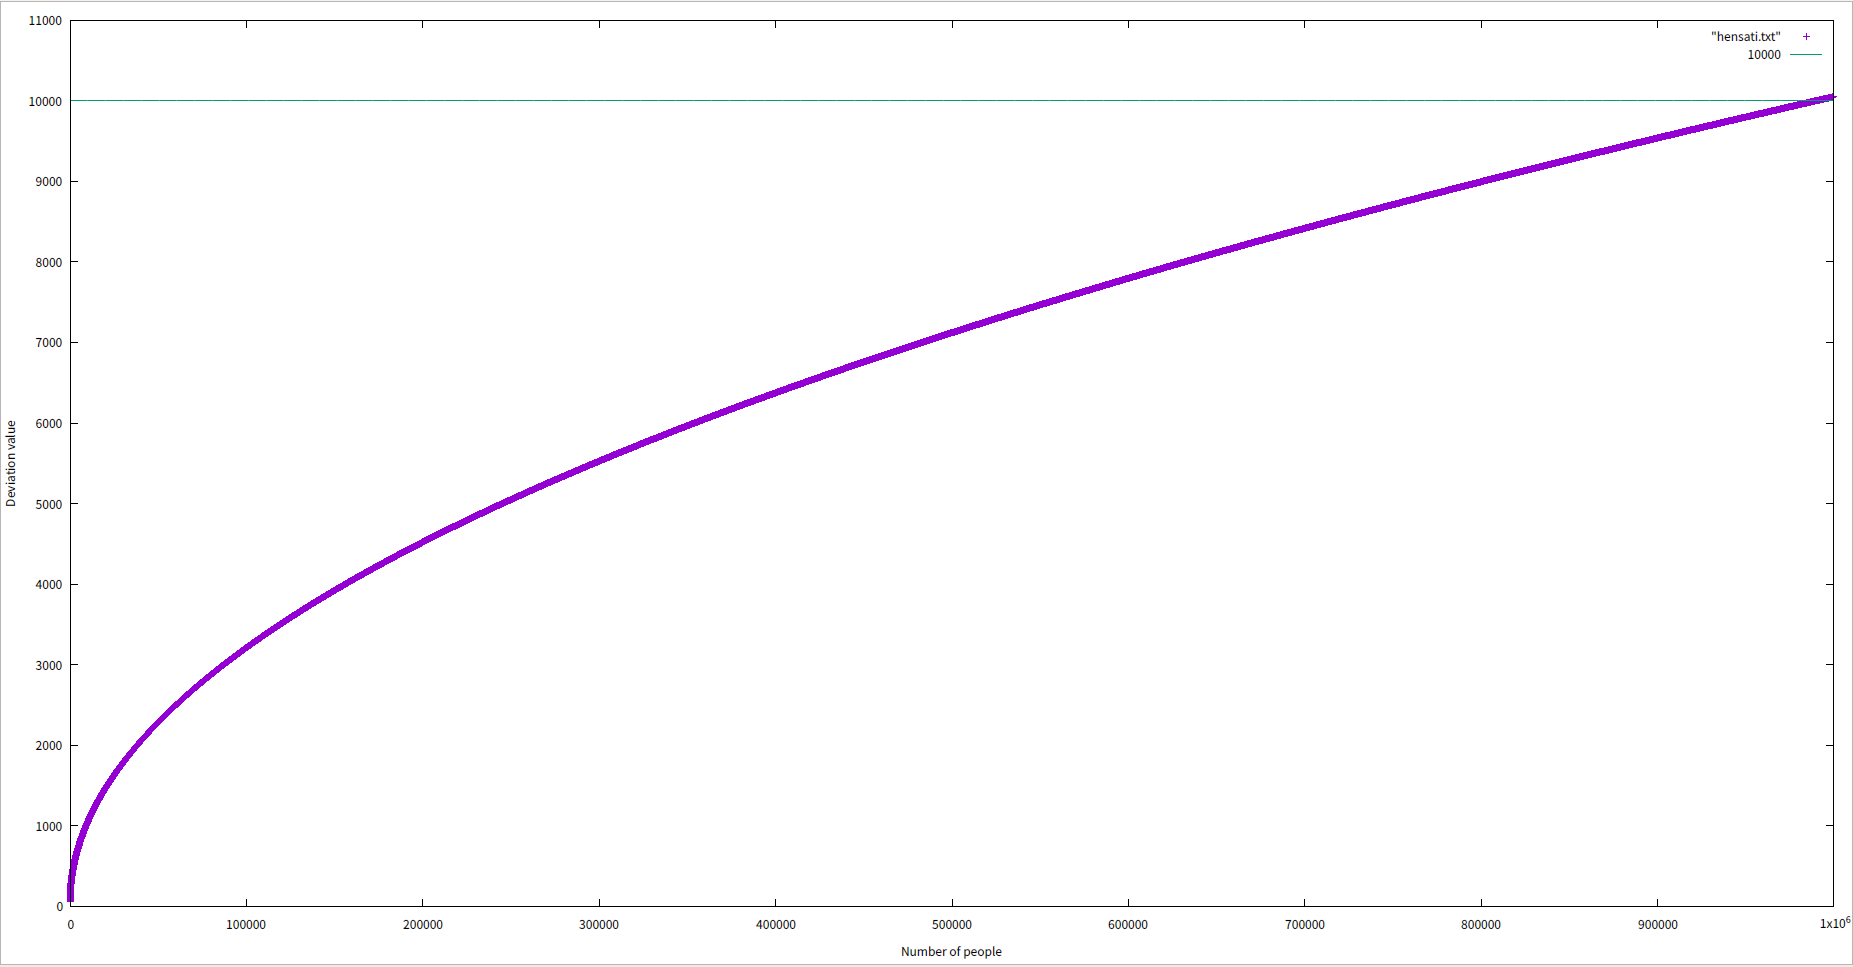
\includegraphics[width=10cm]{image/hensati2.png}
\end{figure}
\begin{center}
  図1 2人から1000000人まで増やした図
\end{center}

\begin{table}[H]
  \begin{center}
    \caption{初めと終わりの偏差値}
    \begin{tabular}{c|c}
      人数 & 偏差値 \\ \hline \hline
      2人 & 60 \\ \hline
      1002人 & 366.402 \\ \hline
      2002人 & 497.348 \\ \hline
      3002人 & 597.832 \\ \hline
      4002人 & 682.55 \\ \hline
            &        \\ \hline
      996002人 & 10030.5 \\ \hline
      997002人 & 10035.5 \\ \hline
      998002人 & 10040.5 \\ \hline
      999002人 & 10045.5 \\ \hline
      1000000人 & 10050.5 \\ \hline
    \end{tabular}
  \end{center}
\end{table}
図1を見ると人数が増えるに連れて偏差値が上がることがわかるが同時に上がるスピードも緩やかになっているのがわかる.それは表1を見ると明らかで、初めは1000人の差で偏差値に100くらいの差があったが1000000人近くになると差がほとんどないということがわかる.

\section{考察・感想}
図1のグラフを見るとだんだんと緩やかになっているのでいつかは収束すると予想する.
偏差値の最大値がほぼ無限になるであろうということを体感することができた。



\end{document}

